\documentclass[tikz]{standalone}
\usepackage[utf8]{inputenc}

\usepackage{tikz}

\usetikzlibrary{shapes.geometric,arrows, fit,positioning}
%\usetikzlibrary{arrows.meta}

\begin{document}

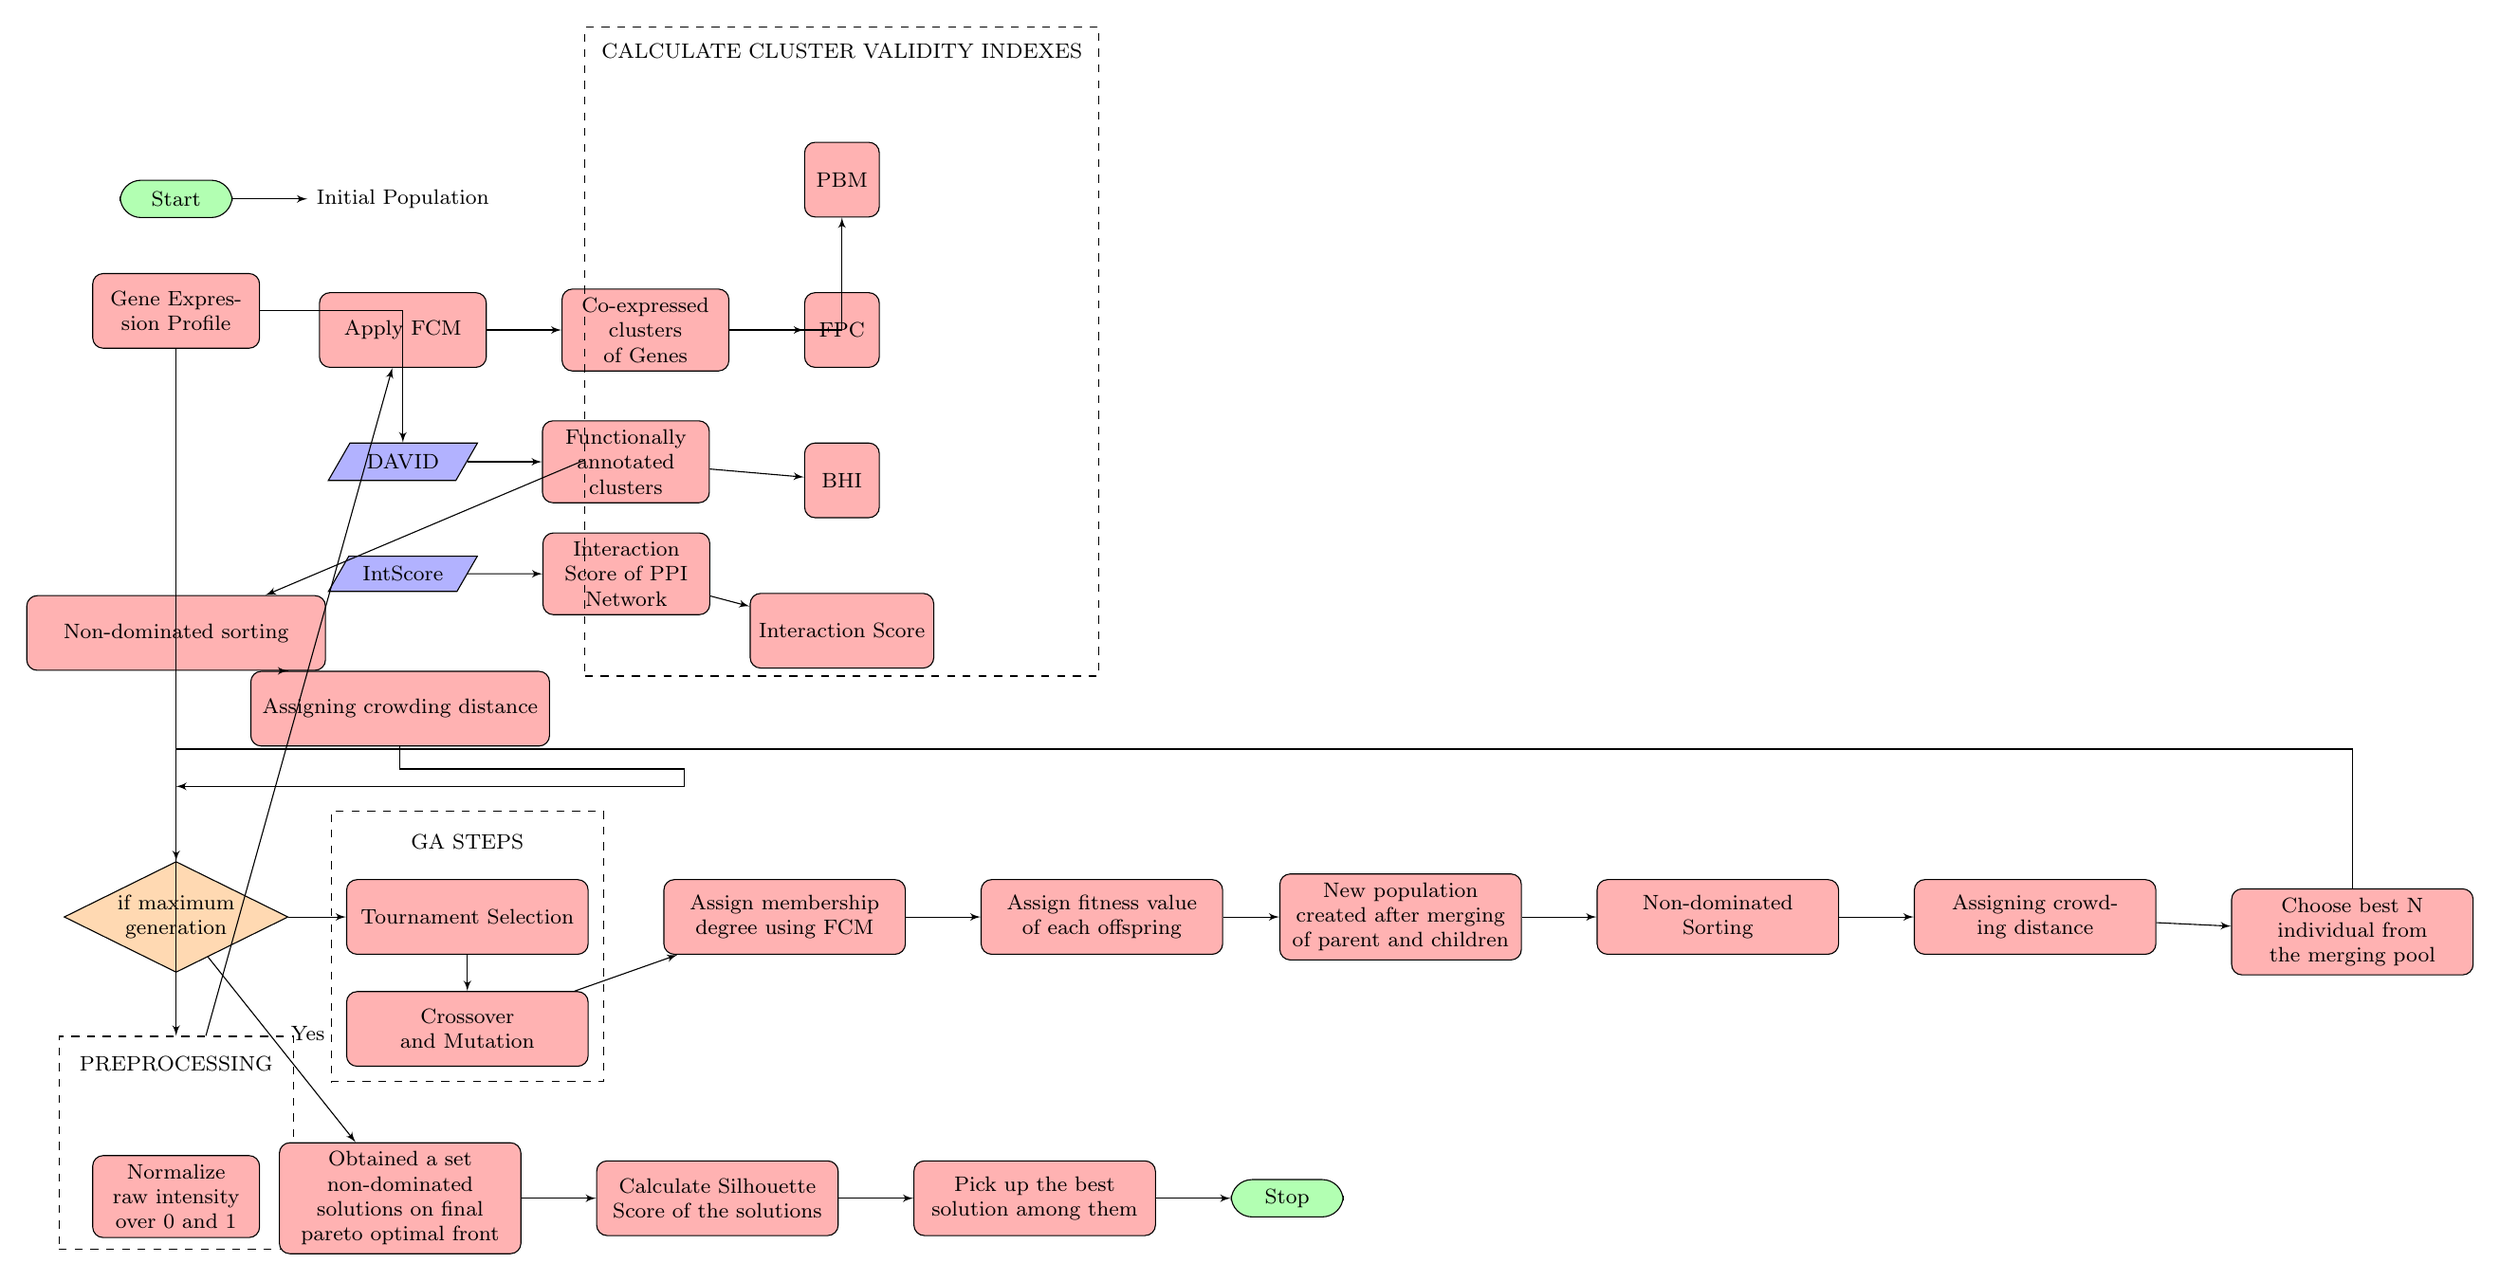
\begin{tikzpicture}[scale=1, auto, every node/.style={font=\footnotesize, >=stealth}]
        \tikzset{
        rblock/.style={draw, shape=rectangle,rounded corners=0.8em,align=center,minimum width=1.5cm,minimum height=0.5 cm, fill=green!30},
        block/.style= {draw, rectangle,rounded corners, align=center,minimum width=2cm,minimum height=1cm,text width= 2cm, fill=red!30},
        block1/.style= {draw, rectangle,rounded corners, align=center,minimum width=3 cm,minimum height=1cm,text width= 3cm, fill=red!30},
        io/.style = {draw, shape=trapezium , trapezium left angle=60, trapezium right angle=120, minimum width=2 cm, text centered, draw=black, fill=blue!30},
        subblock/.style= {draw, rectangle,rounded corners, align=center,minimum width=1cm,minimum height=1cm, fill=red!30},
        superblock/.style= {draw, rectangle,rounded corners, align=center,minimum width=4 cm,minimum height=1cm, fill=red!30},
        decision/.style = {draw,diamond, aspect =2, minimum width=3cm, minimum height=1cm, text centered,text width= 1.8 cm, draw=black, inner sep=0pt, fill=orange!30},
        line/.style = {draw, -latex'}
    }
\node [rblock]  (start) {Start};
\node [block, below of=start, node distance=1.5cm] (Gene_expression_data) {Gene Expression Profile};
\node[right=of start] (AB) {Initial Population};

\node[block,  below=10.8cm of Gene_expression_data] (Normalize){Normalize raw intensity over 0 and 1};
\node[above=of Normalize] (A) {PREPROCESSING};
\node[fit= (A) (Normalize), dashed,draw,inner sep=0.15cm] (Preprocess_box){};

\node [block, below=of AB] (FCM) {Apply FCM};
\node [block, right=of FCM] (Cluster) {Co-expressed clusters of Genes};

\node[io,  below=of FCM] (DAVID){DAVID};
\node [block, right=of DAVID] (FAC) {Functionally annotated clusters};
\node[io,  below=of DAVID] (IntScore){IntScore};
\node [block, right=of IntScore] (PPISCORE) {Interaction Score of PPI Network};
\node [subblock, right=of Cluster] (FPC) {FPC};
\node [subblock,above=of FPC] (PBM) {PBM};
\node [subblock,below=of FPC] (BHI) {BHI};
\node [subblock,below=of BHI] (InteractionScore) {Interaction Score};
\node[above=of PBM] (B) {CALCULATE CLUSTER VALIDITY INDEXES};
\node[fit= (FPC) (PBM) (BHI) (InteractionScore)(B), dashed,draw,inner sep=0.1cm] (Fitness function){};
\node [superblock, below=3.3cm of Gene_expression_data] (NDS1) {Non-dominated sorting};
\node [superblock, below=0pt of NDS1, xshift=3cm] (CROWD1) {Assigning crowding distance};
\node[decision,  above=of A] (Maxgen){if maximum generation};
\node [block1, below=5.3cm of CROWD1] (NDS2) {Obtained a set non-dominated solutions on final pareto optimal front};
\node [block1, right=of NDS2] (Silhouette) {Calculate Silhouette Score of the solutions};
\node [block1, right=of Silhouette] (Bestsol) {Pick up the best solution among them};
\node [rblock, right=of Bestsol] (Stop) {Stop};
\node [block1, right of=Maxgen, node distance=3.9 cm] (tournament) {Tournament Selection};
\node [block1, below of=tournament, node distance=1.5 cm] (Crossover) {Crossover and Mutation};
\node[above of = tournament] (GAS) {GA STEPS};
\node[fit= (GAS) (tournament) (Crossover), dashed,draw,inner sep=0.2cm] (GASteps){};
\node [block1, right=of tournament] (FCM1) {Assign membership degree using FCM};
\node [block1, right=of FCM1] (Fitness) {Assign fitness value of each offspring};
\node [block1, right of=Fitness, node distance=4 cm] (Newpop) {New population created after merging of parent and children};
\node [block1, right=of Newpop] (NDS3) {Non-dominated Sorting};
\node [block1, right=of NDS3] (CROWD2) {Assigning crowding distance};
\node [block1, right=1cm of CROWD2, yshift=-2mm] (nextpop) {Choose best N individual from the merging pool};
\node [coordinate, below right =0.3cm and 1.8 cm of CROWD1] (below) {};  %% Coordinate on right and middle
\node [coordinate,above left =1cm and 1 cm of Maxgen] (top) {};  %% Coordinate on left and middle
\node [coordinate, above =1cm of Maxgen] (top1) {};  %% Coordinate on right and middle
 \node [coordinate,above  =1.5 cm of Maxgen] (top2) {};   

\path [line] (start) -- (AB);
\path [line] (Gene_expression_data) -- (Preprocess_box);
\path [line] (Gene_expression_data) -| (DAVID);
\path [line] (Preprocess_box) -- (FCM);
\path [line] (FCM) -- (Cluster);
\path [line] (Cluster) -- (FPC);
\path [line] (Cluster) -| (PBM);
\path [line] (DAVID) -- (FAC);
\path [line] (FAC) -- (BHI);
\path [line] (IntScore) -- (PPISCORE);
\path [line] (PPISCORE) -- (InteractionScore);
\path [line] (Fitness function) -- (NDS1);
\path [line] (NDS1) -- (CROWD1);
\path [line] (Maxgen) -- (NDS2)node[auto,midway] {Yes};
\path [line] (NDS2) -- (Silhouette);
\path [line] (Silhouette) -- (Bestsol);
\path [line] (Bestsol) -- (Stop);
\path [line] (Maxgen) -- (tournament);
\path [line] (tournament) -- (Crossover);
\path [line] (Crossover) -- (FCM1);
\path [line] (FCM1) -- (Fitness);
\path [line] (Fitness) -- (Newpop);
\path [line] (Newpop) -- (NDS3);
\path [line] (NDS3) -- (CROWD2);
\path [line] (CROWD2) -- (nextpop);
\path [line] (CROWD1) |-(below)|-(top1);
\path [line] (nextpop) |-(top2)--(Maxgen);

\end{tikzpicture}
\end{document}
